\documentclass [a4]{article}
\usepackage[utf8]{inputenc}
\usepackage[french]{babel}
\usepackage{amssymb}
\usepackage{graphicx}
\author{Clément Caumes}
\title{Mon support de cours de méthodologie}
\date {\today}

\begin{document}
\maketitle 
\section{Introduction}
\section{Enoncés des exercices}
\subsection{Poker}
Combien de \textbf{mains} de 5 cartes sont possibles avec {\tiny un jeu} de 52 cartes ? Combien avec 2 as {\huge exactement} ?
\subsection{Si vous répondez mal, gare...}
Un père {\large logicien} dit à son fils \textsf{fais tes devoirs ou je te colle une baffe.} Le fils se dépêche de faire ses devoirs et retourne 
annoncer à son père qu'il les a fini. Celui-ci lui dit c'est très bien et \texttt{lui colle une baffe.} \textit{Le père est il cohérent avec ses déclarations?}
\textbf{Approuvez-vous ses méthodes pédagogiques ?}
\subsection{Tables de vérités}
Ecrire les tables de vérité de $A \Rightarrow B$ et de $\urcorner B \Rightarrow \urcorner A.$ Que constatez vous ?
\section{Corrections des exercices}
\subsection{Poker}
Le nombre de mains de 5 cartes au poker vaut : 

\subsection{Si vous répondez mal, gare...}
\begin{figure}[h]
\centering
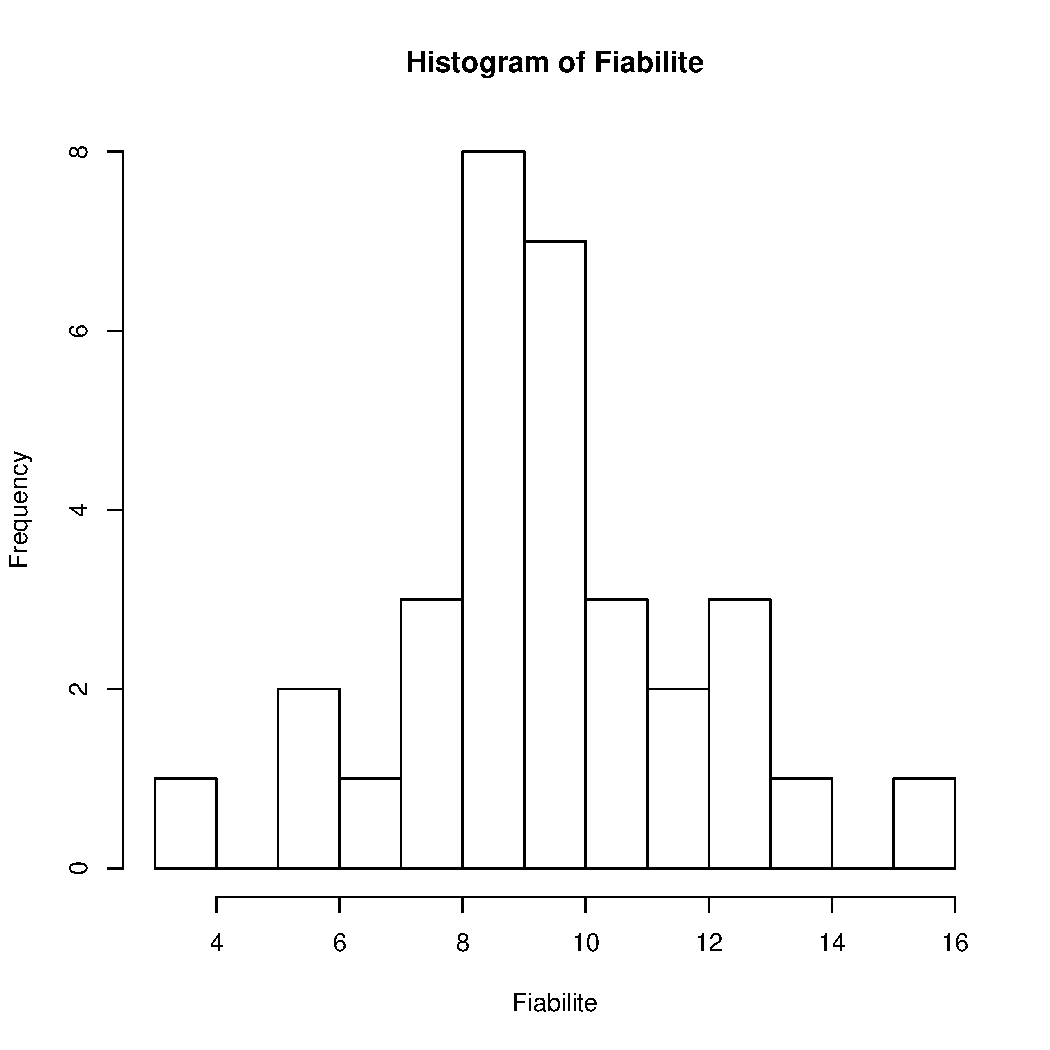
\includegraphics[scale=0.5]{graphe5.pdf}
\caption{Histogramme du R}
\end{figure}
\subsection{Tables de vérités}

\section{Conclusion}
\end{document}

